I dette afsnit bliver der undersøgt hvor udbredt det er at give lommepenge til sine børn, og hvor mange penge de får. Det bliver også undersøgt, om der er pligter forbundet med udleveringen af lommepenge.\\
\\
Fællesforeningen for Danmarks Brugsforeninger (FDB), har lavet en undersøgelse, der bl.a. kigger på hvor mange børn der får lommepenge, og om der også hører pligter med. \cite{FDB1} Undersøgelsen omfatter 1.999 respondenter, og er lavet i 2011.
Ifølge FDB, får lidt over halvdelen (51\%) af de danske børn mellem 3 og 17 år lommepenge. Søjlediagrammet figur \ref{FaarBarnLommepenge} illustrerer forældres svar på, om deres børn får lommepenge. Det store spring, sker fra børn mellem 6 og 8 år, hvor 38\% får lommepenge, til børn mellem 9 og 11 år, hvor 75\% får lommepenge. Det er specielt omkring 9-års alderen, at børnene begynder at få lommepenge. \\
\\
Syv ud af 10 forældre svarer, at der er pligter der skal udføres, for at få lommepenge. Heraf siger halvdelen at der bliver skåret i lommepengene hvis pligterne ikke bliver udført. Af de forældre der giver deres børn lommepenge, siger 59\%, at der kan tjenes ekstra penge, ved at udføre ekstraopgaver.
Ifølge undersøgelsen, modtager et barn der får lommepenge i gennemsnit 69,50 kr om ugen.\\
\\
En undersøgelse fra Nordea, viser at de børn med flest pligter, er dem mellem 9 og 14 år. Ansvarsområder kan være fx kæledyr, madlavning/indkøb, opvask, skraldespand, lektier og oprydning på værelset. \cite{Nordea1}\\
\\
Rigtig mange børn får lommepenge, og mange af børnene skal udføre pligter for pengene. Dette må give børnene en meget basal forståelse for økonomi, da de ved at udføre pligter, der kan ses som "arbejde", modtager penge. Disse penge, kan de så selv benytte til at købe varer i butikker. Denne sammenhæng bliver endda endnu tydeligere for de børn der kan tjene ekstra penge, ved at udføre flere pligter/arbejde for deres forældre.

Men ifølge afsnit \ref{UvidendeUnge} er det ikke nok, til at give børn en bred nok forståelse for økonomi, da de alligevel ender med at skylde en masse penge. Derfor vil der blive kigget på, om det kan med et nytænkt lommepenge system hjælpe børn og unge til at få en bedre forståelse for økonomi, herunder opsparing, renter og måske også lån.

Med alle de børn, der allerede får lommepenge, kan man se at der er gode muligheder for, at lære børn mere om økonomi. Dette kunne f.eks. opnås ved et lommepenge system som gør brug af opsparing og renter, eller andre økonomiske elementer fra den virkelige verden, for så derved at lære børnene omkring økonomi.
\begin{figure}[htb]
\centering
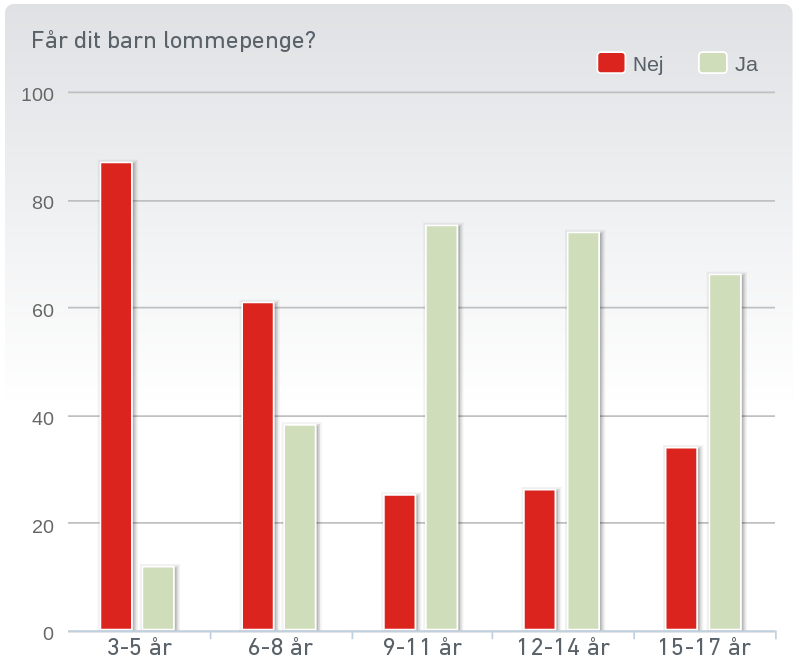
\includegraphics[width=0.6\textwidth]{Billeder/FaarBarnLommepenge.png}
\caption{Forældres svar på spørgsmålet '\textit{Får dit barn lommepenge?}'}
\label{FaarBarnLommepenge}
\end{figure}
